\documentclass[10pt,makeidx]{beamer}



\mode<presentation>
{
 \usetheme{Boadilla}
\pagestyle{empty}

\setbeamerfont*{frametitle}{size=\normalsize,series=\bfseries}
\setbeamerfont*{block}{size=\normalsize,series=\bfseries}
%\setbeamertemplate{blocks}[rounded][shadow=true]
}


\usepackage{epsfig,epstopdf}
\usepackage{etex}
% \usepackage{helvet}
\usepackage{amsmath, amssymb}
\usepackage{color}
\usepackage{asymptote}
\usepackage{mathrsfs}
\usepackage{dsfont}
\usepackage{makeidx}
\usepackage{multido}
\usepackage{adjustbox}
\usepackage{cancel}

\usepackage{pst-sigsys,pst-plot,pstricks-add}
\usepackage{pst-pdf}

\usepackage[american voltages, american currents,siunitx]{circuitikz}
%\sisetup{load=derived} % loading \siemens


\makeatletter
% create the shape
\pgfcircdeclarebipole{}{\ctikzvalof{bipoles/interr/height 2}}{spst}{\ctikzvalof{bipoles/interr/height}}{\ctikzvalof{bipoles/interr/width}}{

    \pgfsetlinewidth{\pgfkeysvalueof{/tikz/circuitikz/bipoles/thickness}\pgfstartlinewidth}

    \pgfpathmoveto{\pgfpoint{\pgf@circ@res@left}{0pt}}
    \pgfpathlineto{\pgfpoint{.6\pgf@circ@res@right}{\pgf@circ@res@up}}
    \pgfusepath{draw}   
}

% make the shape accessible with nice syntax
\def\pgf@circ@spst@path#1{\pgf@circ@bipole@path{spst}{#1}}
\tikzset{switch/.style = {\circuitikzbasekey, /tikz/to path=\pgf@circ@spst@path, l=#1}}
\tikzset{spst/.style = {switch = #1}}
\makeatother





\definecolor{links}{HTML}{2A1B81}
\hypersetup{colorlinks,linkcolor=,urlcolor=links}

\def\nn{\nonumber}

\definecolor{links}{HTML}{2A1B81}
\hypersetup{colorlinks,linkcolor=,urlcolor=links}


\title[]{RLC Circuits}
\author[\textcolor{blue}{Systems and Circuits}]{\textcolor{darkblue}{Pablo M. Olmos} (olmos@tsc.uc3m.es)\\ \textcolor{darkblue}{Emilio Parrado} (emipar@tsc.uc3m.es)}
\institute{\textcolor{white}{UC3M}}

\definecolor{darkblue}{rgb}{0.0, 0.0, 0.40}
\setbeamercolor{title}{fg=darkblue}
\setbeamercolor{frametitle}{fg=darkblue}
\definecolor{darkgreen}{rgb}{0.0, 0.4, 0.0}%


\AtBeginSection[]
{
  \begin{frame}<beamer>{Index}
    \tableofcontents[currentsection,currentsubsection]
  \end{frame}
}

\begin{document}
\frame{
\titlepage
\thispagestyle{empty}
\begin{center}

\includegraphics[scale=0.05]{Figures/uc3m-logo.pdf}
\end{center}
}

\section{General solution of the Second-order  differential equation}


\frame{
\frametitle{Second order  linear differential equation with constant coefficients}
Compute $y(t)$ such that $y(t_0)=y_0$, $\frac{dy(t)}{dt}|_{t=t_0}=y_1$ if 
%\begin{align}\nn
%A\frac{dx(t)}{dt}+Bx(t)=C
%\end{align}
%where $A$, $B$ and $C$ are constants.
%
\begin{align}\nn
\frac{d^2y(t)}{dt^2}+2\alpha\frac{dy(t)}{dt}+\omega_0^2 y(t)=\gamma
\end{align}
where  $\alpha$, $\omega_0^2$ are real constants.


}

\frame{
\frametitle{Second order  linear differential equation with constant coefficients}
Compute $y(t)$ such that $y(t_0)=y_0$, $\frac{dy(t)}{dt}|_{t=t_0}=y_1$ if 
%\begin{align}\nn
%A\frac{dx(t)}{dt}+Bx(t)=C
%\end{align}
%where $A$, $B$ and $C$ are constants.
%
\begin{align}\nn
\frac{d^2y(t)}{dt^2}+2\alpha\frac{dy(t)}{dt}+\omega_0^2 y(t)=\gamma
\end{align}
where  $\alpha$, $\omega_0^2$ are real constants.

\begin{alertblock}{Characteristic equation:}
$s_1$ and $s_2$ are the roots of the equation
\begin{align*}
s^2+ 2\alpha s+\omega_0^2=0
\end{align*}
Thus
\begin{align*}
s_1=-\alpha+\sqrt{\alpha^2-\omega_0^2}\qquad s_2=-\alpha-\sqrt{\alpha^2-\omega_0^2}
\end{align*}
\end{alertblock}

}

\frame{
\frametitle{Case $\alpha>\omega_0$: $s_1$ and $s_2$ are negative real constants}

\begin{block}{}
\begin{align*}
y(t)=A_1 \text{e}^{s_1 (t-t_0)}+ A_2 \text{e}^{s_2 (t-t_0)}+\frac{\gamma}{\omega^2_0}\qquad t\geq t_0,
\end{align*}
where $A_1$ and $A_2$ can be found using the initial conditions.
\end{block}

}


\frame{
\frametitle{Exercise}

Let $x(t)= 3u(t)$ be the input signal to a system defined by the following input/output relationship:
\begin{align*}
\frac{d^2y(t)}{dt^2}+6\frac{dy(t)}{dt}+5y(t)=x(t),
\end{align*}
where $y(t)$ is the output signal. If we know that $y(0)=0$ and  $\frac{dy(t)}{dt}|_{t=0}=0$, compute and plot $y(t)$.

}

\frame{
\frametitle{Sol.}

For $t\geq 0$, the equation that gives the output is a second-order differential equation of the form 
\begin{align*}
\frac{d^2y(t)}{dt^2}+6\frac{dy(t)}{dt}+5 y(t)=3\qquad t\geq 0
\end{align*}

\begin{alertblock}{}
\begin{align*}
s^2+ 6 s+5=0\Rightarrow s_1=-3+\sqrt{9-5}=-1, s_2=-3-\sqrt{2}=-5
\end{align*}
\end{alertblock}

\begin{exampleblock}{}
\begin{align*}
y(t)=A_1  \text{e}^{-t}+ A_2 \text{e}^{-5t}+\frac{3}{5}\qquad t\geq 0
\end{align*}
\end{exampleblock}

Using the initial conditions we find $A_1=\frac{-3}{5}$ and $A_2=\frac{3}{25}$. 

}

\frame{

\begin{figure}
\centering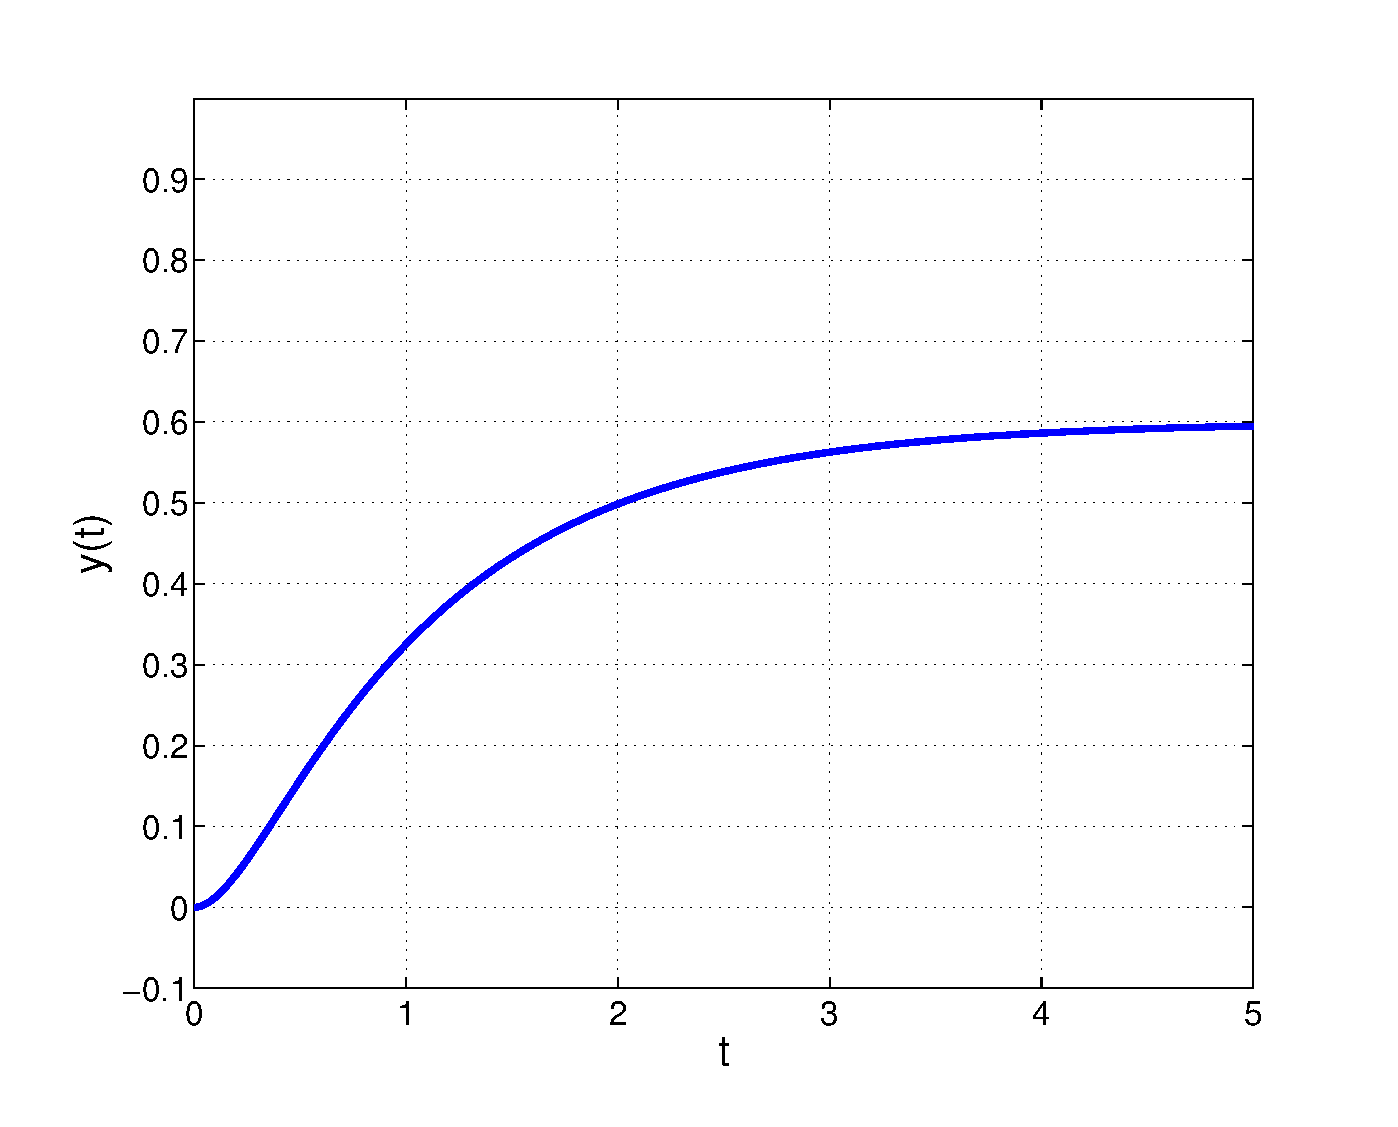
\includegraphics[scale=0.4]{Figures/overdamped.eps}
\end{figure}

The response of this system to the unit step is said to be \emph{overdamped}.

}






\frame{
\frametitle{Case $\alpha<\omega_0$: $s_1$ and $s_2$ are complex}

\begin{align*}
s_1=-\alpha+j\sqrt{\omega_0^2-\alpha^2}\qquad s_2=-\alpha-j\sqrt{\omega_0^2-\alpha^2}
\end{align*}
Define $\omega_d\doteq \sqrt{\omega_0^2-\alpha^2}$.

\begin{block}{}
\begin{align*}
y(t)=B_1 \text{e}^{-\alpha (t-t_0)}\cos(\omega_d (t-t_0))+B_2 \text{e}^{-\alpha (t-t_0)}\sin(\omega_d (t-t_0))+\frac{\gamma}{\omega^2_0} \qquad t\geq t_0,
\end{align*}
where $B_1$ and $B_2$ can be found using the initial conditions.
\end{block}

\begin{alertblock}{$\alpha=0$}
Oscillation around $\gamma/\omega_0^2$!! The solution \textbf{does not} converge to a constant value in the limit $t\rightarrow\infty$!!!
\end{alertblock}

}



\frame{
\frametitle{Exercise}

Let $x(t)= 3u(t)$ be the input signal to a system defined by the following input/output relationship:
\begin{align*}
\frac{d^2y(t)}{dt^2}+\frac{dy(t)}{dt}+5 y(t)=x(t),
\end{align*}
where $y(t)$ is the output signal. If we know that $y(0)=0$ and  $\frac{dy(t)}{dt}|_{t=0}=0$, compute and plot $y(t)$.

}

\frame{
\frametitle{Sol.}

For $t\geq 0$, the equation that gives the output is a second-order differential equation of the form 
\begin{align*}
\frac{d^2y(t)}{dt^2}+\frac{dy(t)}{dt}+5 y(t)=3\qquad t\geq 0
\end{align*}

\begin{alertblock}{}
\begin{align*}
s^2+  s+5=0\Rightarrow s_1=-0.5+j\sqrt{4.75}, s_2=-0.5-j\sqrt{4.75}
\end{align*}
\end{alertblock}

\begin{exampleblock}{}
\begin{align*}
y(t)=B_1 \text{e}^{-\frac{t}{2}}\cos(\sqrt{4.75} t)+B_2 \text{e}^{-\frac{t}{2}}\sin(\sqrt{4.75} t)+\frac{3}{5} \qquad t\geq 0
\end{align*}
\end{exampleblock}

Using the initial conditions we find $B_1=\frac{-3}{5}$ and $B_2=\frac{3}{10\sqrt{4.75}}$ (check!). 

}


\frame{

\begin{figure}
\centering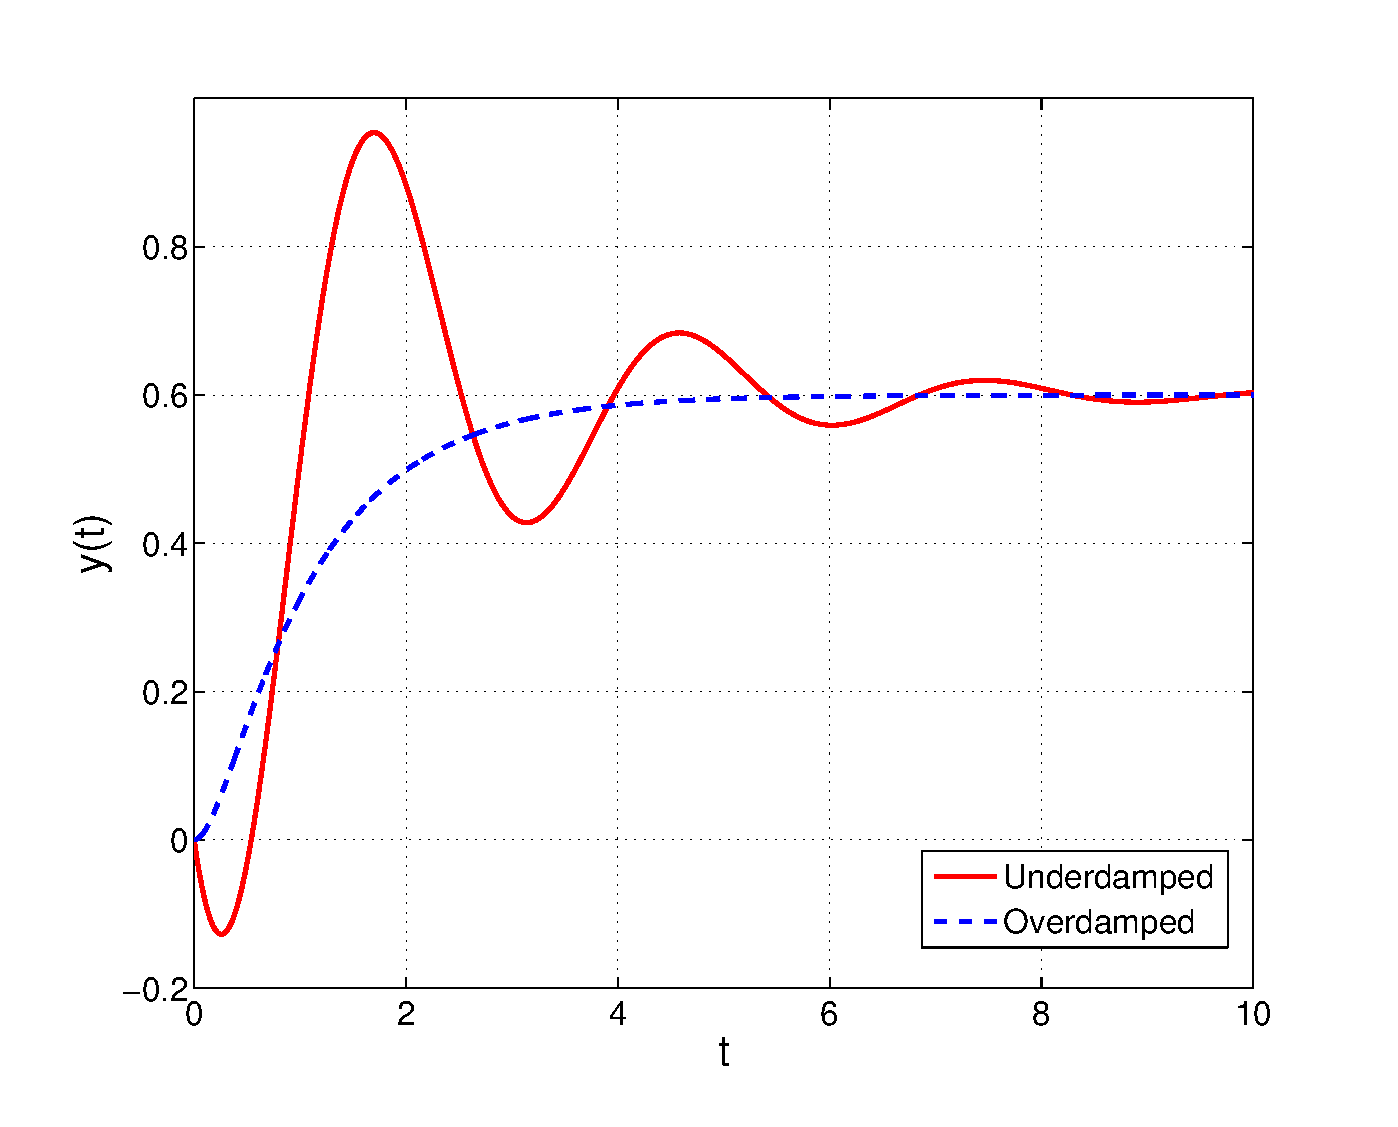
\includegraphics[scale=0.4]{Figures/underdamped.eps}
\end{figure}

The response of this system to the unit step is said to be \emph{underdamped}.

}



\frame{
\frametitle{Case $\alpha=\omega$: $s_1=s_2=-\alpha$}

\begin{block}{}
\begin{align*}
y(t)=(D_1+D_2 (t-t_0)) \text{e}^{-\alpha (t-t_0)} \qquad t\geq t_0,
\end{align*}
where $D_1$ and $D_2$ can be found using the initial conditions.
\end{block}


}


\frame{
\frametitle{Exercise}

Let $x(t)= 3u(t)$ be the input signal to a system defined by the following input/output relationship:
\begin{align*}
\frac{d^2y(t)}{dt^2}+2\sqrt{5}\frac{dy(t)}{dt}+5y(t)=x(t),
\end{align*}
where $y(t)$ is the output signal. If we know that $y(0)=0$ and  $\frac{dy(t)}{dt}|_{t=0}=0$, compute and plot $y(t)$.

}

\frame{
\frametitle{Sol.}

For $t\geq 0$, the equation that gives the output is a second-order differential equation of the form 
\begin{align*}
\frac{d^2y(t)}{dt^2}+2\sqrt{5}\frac{dy(t)}{dt}+5 y(t)=3\qquad t\geq 0
\end{align*}

\begin{alertblock}{}
\begin{align*}
s^2+ 2\sqrt{5} s+5=0\Rightarrow s_1=s_2=-\sqrt{5}
\end{align*}
\end{alertblock}

\begin{exampleblock}{}
\begin{align*}
y(t)=(D_1+D_2 t) \text{e}^{-\sqrt{5} t} +\frac{3}{5}\qquad t\geq t_0
\end{align*}
\end{exampleblock}

Using the initial conditions we find $D_1=\frac{-3}{5}$ and $D_2=\frac{-3}{\sqrt{5}}$. 

}

\frame{

\begin{figure}
\centering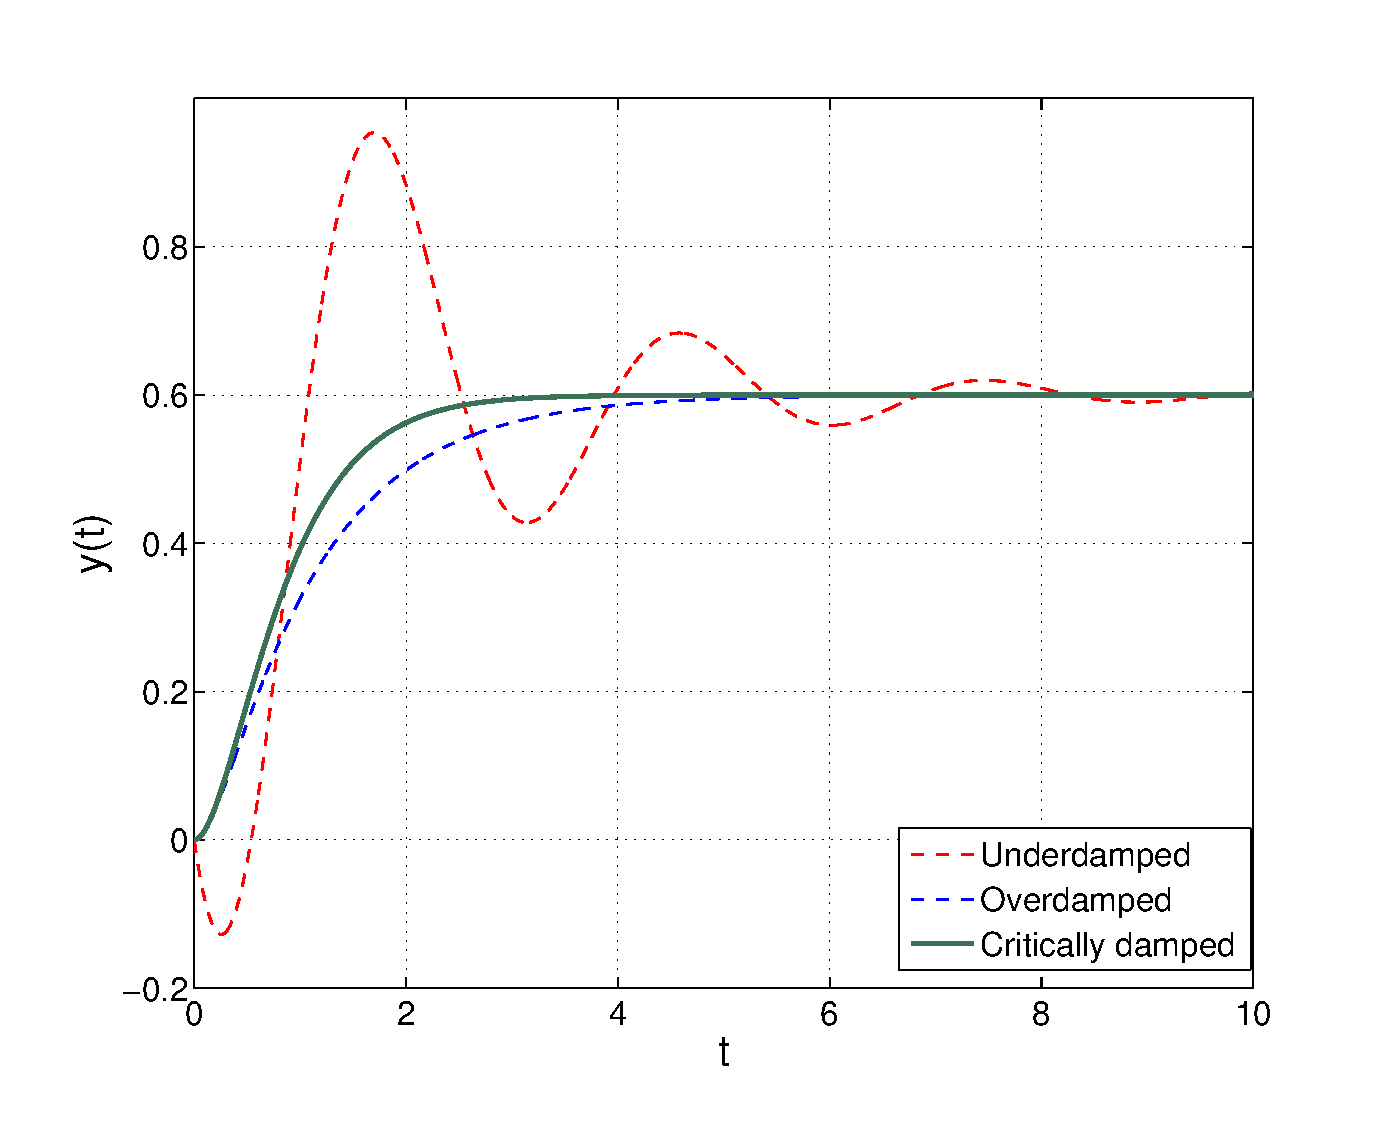
\includegraphics[scale=0.4]{Figures/critically_damped.eps}
\end{figure}

The response of this system to the unit step is said to be \emph{critically damped}.

}

\section{RLC circuits}


\frame{
\frametitle{Example}

\begin{center}
\begin{circuitikz}[] \draw[black]
(-2,0) to[short,i>=$i(t)$] (-2,2)
(-2,2) to[L=$L$] (0,2)
to[R=$R$] (2,2)
to[C=$C$] (2,0)
(2,2) to[short,-*] (5,2)
(2,0) to[short,-*] (5,0)
(2,0) to[short](-2,0)
(5,2) to[open,v<=$V_C(t)$] (5,0);
\end{circuitikz}
\end{center}

\begin{block}{}
If $i(0)=i_0$ and $\frac{\partial i(t)}{\partial t}|_{t=0}=i'_0$, determine the differential equation for the current $i(t)$ for $t\geq 0$.
\end{block}

}

\frame{
\frametitle{Sol.}

\begin{center}
\begin{circuitikz}[] \draw[black]
(-2,0) to[short,i>=$i(t)$] (-2,2)
(-2,2) to[L=$L$,v<=$v_L(t)$] (0,2)
to[R=$R$] (2,2)
to[C=$C$] (2,0)
(2,2) to[short,-*] (5,2)
(2,0) to[short,-*] (5,0)
(2,0) to[short](-2,0)
(5,2) to[open,v<=$V_C(t)$] (5,0);
\end{circuitikz}
\end{center}


 KVL in the loop:


\begin{align*}
v_L(t)+i(t)R+V_C(t)=0
\end{align*}


 We express all terms as a function of $i(t)$:


\begin{align*}
v_L(t)&=L\frac{\partial i(t)}{\partial t}\\
v_C(t)&=\frac{1}{C}\int_{-\infty}^{t} i(\tau) d\tau
\end{align*}

}

\frame{
Thus
\begin{align*}
L\frac{\partial i(t)}{\partial t}+i(t)R+\frac{1}{C}\int_{-\infty}^{t} i(\tau) d\tau=0
\end{align*}

This equation can be transformed into a second order differential equation by computing the time-derivative at both sides of the equation...

\begin{align*}
L\frac{\partial^2 i(t)}{\partial t^2}+\frac{\partial i(t)}{\partial t}R+\frac{1}{C}i(t)=0
\end{align*}

To find the solution for $i(t)$ $t\geq 0$ using our "recipe", we divide by $L$ so the coefficient for $\frac{\partial^2 i(t)}{\partial t^2}$ is one...

\begin{align*}
\frac{\partial^2 i(t)}{\partial t^2}+\frac{R}{L} \frac{\partial i(t)}{\partial t}+\frac{1}{LC}i(t)=0
\end{align*}

}

\frame{
\begin{block}{}
\begin{columns}
\begin{column}{0.4\textwidth}
\begin{align}\nn
\frac{d^2y(t)}{dt^2}+2\alpha\frac{dy(t)}{dt}+\omega_0^2 y(t)=\gamma,
\end{align}
\end{column}
\begin{column}{0.25\textwidth}
\begin{align*}
s^2+ 2\alpha s+\omega_0^2=0,
\end{align*}
\end{column}
\begin{column}{0.35\textwidth}
\begin{align*}
s_{1,2}=-\alpha\pm\sqrt{\alpha^2-\omega_0^2}
\end{align*}
\end{column}
\end{columns}
\end{block}

We identify terms

\begin{align*}
\frac{\partial^2 i(t)}{\partial t^2}+\frac{R}{L} \frac{\partial i(t)}{\partial t}+\frac{1}{LC}i(t)=0\quad \Rightarrow \omega_0^2=\frac{1}{LC}, 2\alpha=R/L.
\end{align*}

\begin{exampleblock}{$s_{1,2}=-\frac{R}{2L}\pm\sqrt{\frac{R^2}{4L^2}-\frac{1}{LC}}$}
\begin{itemize}
\item $R>2\sqrt{\frac{L}{C}}\rightarrow$ real (negative) roots. Overdamped solution.
\item $R<2\sqrt{\frac{L}{C}}\rightarrow$ complex roots. Underdamped solution.
\item $R=2\sqrt{\frac{L}{C}}\rightarrow$ 2 equal roots. Critically damped solution.
\item $R=0\rightarrow$ Oscillation.
\end{itemize}
\end{exampleblock}



}

\frame{
\frametitle{Example}

\begin{center}
\begin{circuitikz}[] \draw[black]
(-2,0) to[I,i>=$I_s$] (-2,3)
to[short](0,3)
to[cspst,l^=\mbox{t=0}] (1,3)
to[short](6,3)
(-1,3) to[ospst, l^ = \mbox{t = 0}] (-1,0)
(1,3) to[L=$L$,i>=$i_L(t)$] (1,0)
(4,3) to[C=$C$,v<=$v_0(t)$] (4,0)
(6,3) to[R=$R$] (6,0)
to [short] (-2,0);
\end{circuitikz}
\end{center}

\begin{block}{}
Determine the differential equation for the current $i_L(t)$ for $t\geq 0$.
\end{block}

\begin{alertblock}{}
Determine the differential equation for the voltage  $v_0(t)$ for $t\geq 0$.
\end{alertblock}

}

\frame{

\begin{center}
\begin{circuitikz}[] \draw[black]
(-2,0) to[I,i>=$I_s$] (-2,3)
to[short](0,3)
to[short] (1,3)
to[short](6,3)
(-1,3) to[ospst] (-1,0)
(1,3) to[L=$L$,i>=$i_L(t)$] (1,0)
(4,3) to[C=$C$,v<=$v_0(t)$,i>=$i_C(t)$] (4,0)
(6,3) to[R=$R$,i>=$i_R(t)$] (6,0)
to [short] (-2,0)
(3,0) node[ground] {};
\end{circuitikz}
\end{center}


\begin{align*}
\text{ KCL: } I_s=i_L(t)+i_C(t)+i_R(t)
\end{align*}

\begin{itemize}
\item Inductor: $v_0(t)=L\frac{\partial i_L(t)}{\partial t}$
\item Resistor: $i_R(t)=v_0(t)/R=\frac{L}{R}\frac{\partial i_L(t)}{\partial t}$
\item Capacitor: $i_C(t)=C\frac{\partial v_0(t)}{\partial t}=CL \frac{\partial^2 i_L(t)}{\partial^2 t} $

\end{itemize}

}

\frame{
\begin{block}{}
\begin{columns}
\begin{column}{0.4\textwidth}
\begin{align}\nn
\frac{d^2y(t)}{dt^2}+2\alpha\frac{dy(t)}{dt}+\omega_0^2 y(t)=\gamma,
\end{align}
\end{column}
\begin{column}{0.25\textwidth}
\begin{align*}
s^2+ 2\alpha s+\omega_0^2=0,
\end{align*}
\end{column}
\begin{column}{0.35\textwidth}
\begin{align*}
s_{1,2}=-\alpha\pm\sqrt{\alpha^2-\omega_0^2}
\end{align*}
\end{column}
\end{columns}
\end{block}

Therefore
\begin{align*}
&CL \frac{\partial^2 i_L(t)}{\partial^2 t} + \frac{L}{R}\frac{\partial i_L(t)}{\partial t}+i_L(t)=I_s\\\\
%&\Rightarrow \frac{\partial^2 i_L(t)}{\partial^2 t}+ \frac{1}{RC}\frac{\partial i_L(t)}{\partial t}+\frac{1}{CL} i_L(t)=\frac{I_s}{CL}\\
&\Rightarrow \omega_0^2=\frac{1}{LC}, 2\alpha=\frac{1}{RC}, \gamma=\frac{I_s}{CL}
\end{align*}

\begin{exampleblock}{$s_{1,2}=-\frac{1}{2RC}\pm\sqrt{\frac{1}{4(RC)^2}-\frac{1}{LC}}$}
\begin{itemize}
\item $R<\frac{1}{2}\sqrt{\frac{L}{C}}\rightarrow$ real (negative) roots. Overdamped solution.
\item $R>\frac{1}{2}\sqrt{\frac{L}{C}}\rightarrow$ complex roots. Underdamped solution.
\item $R=\frac{1}{2}\sqrt{\frac{L}{C}}\rightarrow$ 2 equal roots. Critically damped solution.
\item $R=\infty\rightarrow$ Oscillation.
\end{itemize}
\end{exampleblock}


}

\frame{
\frametitle{Auxiliary conditions}
We need $i_L(0^+)$ and $\frac{\partial i_L(t)}{\partial t}|_{t=0^+}$. If the circuit has been operating for a long time before the switch is open, then the equivalent circuit is 

\begin{center}
\begin{circuitikz}[] \draw[black]
(-2,0) to[I,i>=$I_s$] (-2,3)
to[short](0,3)
to[open,*-*] (1,3)
to[short](6,3)
(-1,3) to[short] (-1,0)
(1,3) to[short] (1,0)
(4,3) to[open,*-*,v<=$v_0(t)$] (4,0)
(6,3) to[R=$R$,i>=$i_R(t)$] (6,0)
to [short] (-2,0);
\end{circuitikz}
\end{center}

Therefore, $i_L(0^-)=i_L(0^+)=0$ A and $v_0(0^-)=v_0(0^+)=0$ V.  Since $v_0(t)=l\frac{\partial i_L(t)}{\partial t}$, this means 
\begin{align*}
\frac{\partial i_L(t)}{\partial t}|_{t=0^+}=0 \quad \text{A/s}
\end{align*}




}

\frame{

\begin{center}
\begin{circuitikz}[] \draw[black]
(-2,0) to[I,i>=$I_s$] (-2,3)
to[short](6,3)
(-1,3) to[ospst, l^ = \mbox{t = 0}] (-1,0)
(1,3) to[L=$L$,i>=$i_L(t)$] (1,0)
(4,3) to[C=$C$,v<=$v_0(t)$,i>=$i_C(t)$] (4,0)
(6,3) to[R=$R$,i>=$i_R(t)$] (6,0)
to [short] (-2,0)
(3,0) node[ground] {};
\end{circuitikz}
\end{center}

\begin{itemize}
\item If we already have the solution to $i_L(t)$, then $v_0(t)=L\frac{\partial i_L(t)}{\partial t}$.
\item We can directly obtain the differential equation for $v_0(t)$.
\end{itemize}

}

\frame{
\begin{center}
\begin{circuitikz}[] \draw[black]
(-2,0) to[I,i>=$I_s$] (-2,3)
to[short](6,3)
(-1,3) to[ospst, l^ = \mbox{t = 0}] (-1,0)
(1,3) to[L=$L$,i>=$i_L(t)$] (1,0)
(4,3) to[C=$C$,v<=$v_0(t)$,i>=$i_C(t)$] (4,0)
(6,3) to[R=$R$,i>=$i_R(t)$] (6,0)
to [short] (-2,0)
(3,0) node[ground] {};
\end{circuitikz}
\end{center}


\begin{align*}
\text{ KCL: } I_s=i_L(t)+i_C(t)+i_R(t)
\end{align*}

\begin{itemize}
\item Resistor: $i_R(t)=v_0(t)/R$
\item Capacitor: $i_c(t)=C\frac{\partial v_0(t)}{\partial t}$
\item Inductor: $i_L(t)=\frac{1}{L}\int_{-\infty}^{t}v_0(\tau)d\tau$
\end{itemize}

}

\frame{
Therefore
\begin{align*}
I_s=\frac{1}{L}\int_{-\infty}^{t}v_0(\tau)d\tau+C\frac{\partial v_0(t)}{\partial t}+\frac{1}{R}v_0(t)
\end{align*}

If we compute the time-derivative at both sides of the equation

\begin{align*}
\frac{\partial^2 v_0(t)}{\partial t^2}+\frac{1}{RC}\frac{\partial v_0(t)}{\partial t}\frac{1}{LC}v_0(t)=0
\end{align*}

\begin{exampleblock}{$s_{1,2}=-\frac{1}{2RC}\pm\sqrt{\frac{1}{4(RC)^2}-\frac{1}{LC}}$}
\begin{itemize}
\item $R<\frac{1}{2}\sqrt{\frac{L}{C}}\rightarrow$ real (negative) roots. Overdamped solution.
\item $R>\frac{1}{2}\sqrt{\frac{L}{C}}\rightarrow$ complex roots. Underdamped solution.
\item $R=\frac{1}{2}\sqrt{\frac{L}{C}}\rightarrow$ 2 equal roots. Critically damped solution.
\item $R=\infty\rightarrow$ Oscillation.
\end{itemize}
\end{exampleblock}

}



\section{RLC circuits as systems (filters)}

\frame{
\frametitle{RLC circuits as systems}
\begin{center}
\begin{circuitikz}[] \draw[color=red]
(-2,0) to[I,i>=$I_s$, color=red] (-2,3);
\draw[color=black] (-2,3)
to[short](6,3)
(-1,3) to[ospst, l^ = \mbox{t = $t_0$}] (-1,0)
(1,3)  to[R=$R$,i>=$i_R(t)$]  (1,0)
(4,3) to[C=$C$,v<=$v_0(t)$,i>=$i_C(t)$] (4,0);
\draw[color=blue]
(6,3) to[L=$L$,i>=$i_L(t)$, color=blue] (6,0);
\draw[color=black] 
(6,3) to[L=$L$] (6,0)
(6,0)
to [short] (-2,0);
\end{circuitikz}
\end{center}


Differential equation for $i_L(t)$:

\begin{align*}
&\frac{\partial^2 i_L(t)}{\partial^2 t} + \frac{1}{RC}\frac{\partial i_L(t)}{\partial t}+\frac{1}{L}i_L(t)=\frac{ I_s}{LC} u(t-t_0)% \\\\
%&\Rightarrow \omega_0^2=\frac{1}{LC}, 2\alpha=\frac{1}{RC}, \gamma=\frac{I_s}{CL}
\end{align*}

with auxiliary conditions $i_L(t_0) = A$, $\frac{\partial i_L(t)}{\partial t}|_{t=t_0}=B$


We can consider {\color{red} $I_s u(t-t_0)$} as the {\color{red} input} and {\color{blue} $i_L(t)$} as the {\color{blue} output} of a system that is implemented by the RLC circuit. These systems are called \textbf{filters}.

}

\frame{
\frametitle{Filters}
\begin{alertblock}{}
The {\bf system} input/output relationship is given by the differential equation and the auxiliary conditions.
\end{alertblock}
\begin{center}
\begin{pspicture}[](6,2)
   \pssignal(0,1){x}{$I_su(t-t_0)$}
   \psblock(2,1){a}{Filter}
   %\psblock(4,1){b}{$h[n], H(z)$}
   \pssignal(4,1){y}{$i_L(t)$}
   %-----------------
   \psset{arrows=->}
   \ncline{x}{a}  \ncline{a}{y}  %\ncline{b}{y}
\end{pspicture}
\end{center}

We can characterize the system using the properties defined for systems in the first part of the course. In particular, we will discuss the linearity, time-invariance and causality properties of the filter.
}

\frame{
\frametitle{Linearity}
If we put an input current {\color{red} $I_1$} in the source, we will observe a current in the inductor {\color{blue} (system output) $i_1(t)$} such that:
\begin{align*}
&\frac{\partial^2 i_1(t)}{\partial^2 t} + \frac{1}{RC}\frac{\partial i_1(t)}{\partial t}+\frac{1}{L}i_1(t)=\frac{ I_1}{LC} u(t-t_0)% \\\\
%&\Rightarrow \omega_0^2=\frac{1}{LC}, 2\alpha=\frac{1}{RC}, \gamma=\frac{I_s}{CL}
\end{align*}
with auxiliary contidions $i_1(t_0) = A$, $\frac{\partial i_1(t)}{\partial t}|_{t=t_0}=B$

If we consider a different input {\color{red} $I_2$}, the new output current  {\color{green} $i_2(t)$} verifies
\begin{align*}
&\frac{\partial^2 i_2(t)}{\partial^2 t} + \frac{1}{RC}\frac{\partial i_2(t)}{\partial t}+\frac{1}{L}i_2(t)=\frac{ I_2}{LC} u(t-t_0)% \\\\
%&\Rightarrow \omega_0^2=\frac{1}{LC}, 2\alpha=\frac{1}{RC}, \gamma=\frac{I_s}{CL}
\end{align*}
with auxiliary conditions $i_2(t_0) = A$, $\frac{\partial i_2(t)}{\partial t}|_{t=t_0}=B$
}

\frame{
If we consider an input that is the linear combination of the two former inputs {\color{red}$I_3 = aI_1 + bI_2$} the new output {\color{blue} $i_3(t)$} is such that

\begin{align*}
\frac{(aI_1 + b I_2)}{LC}u(t-t_0)=&a\left\{ \frac{\partial^2 i_1(t)}{\partial^2 t} + \frac{1}{RC}\frac{\partial i_1(t)}{\partial t}+\frac{1}{L}i_1(t) \right \} + \\\\
& b\left\{\frac{\partial^2 i_2(t)}{\partial^2 t} + \frac{1}{RC}\frac{\partial i_2(t)}{\partial t}+\frac{1}{L}i_2(t)\right \} 
\end{align*}
\begin{align*}
=\frac{\partial^2  (ai_1(t) +b i_2(t) )}{\partial^2 t} + \frac{1}{RC}\frac{\partial (ai_1(t) +b i_2(t) )}{\partial t}+\frac{1}{L}(ai_1(t) +b i_2(t) )
\end{align*}

Hence, the output is  $i_3(t) = a i_1(t) + b i_2(t)$. 
 
But we have to see what happens with the auxiliary conditions.
}

\frame{
\frametitle{Filter linearity: auxiliary conditions}
The current {\color{blue} $i_3(t)$} must verify
\[
\begin{array}{ccc}  i_3(t_0) & = &A  \\ \frac{\partial i_3(t)}{\partial t}|_{t=t_0}& = & B\end{array} \Rightarrow \begin{array}{ccc}  ai_1(t_0) + bi_2(t_0) & = &A  \\ \frac{\partial (ai_1(t)+bi_2(t))}{\partial t}|_{t=t_0}& = & B \end{array}
\]

On the other hand 
\[
\begin{array}{ccc}  ai_1(t_0) + bi_2(t_0) & = &aA + bA  \\ \frac{\partial (ai_1(t)+bi_2(t))}{\partial t}|_{t=t_0}& = & aB+bB \end{array} 
\]

Putting all together

\[
\begin{array}{ccc}  A & = &(a + b)A  \\ B& = & (a+b)B \end{array} 
\]
which has to be true for any $a$, $b$, hence  $A=B=0$.

\begin{exampleblock}{Linearity condition for a filter}
Null auxiliary conditions!
\end{exampleblock}
}

\frame{
\frametitle{Time Invariancy}
\begin{itemize}
\item $i_L(t)$ is the output when the input is  {\color{red}$I_s u(t-t_0)$}.

\item If we close the switch at $t_1>t_0$, we are essentially delaying the input: {\color{red}$I_s u(t-t_1)$}.

\item For this new input, we know the solution is automatically shifted to $t_1$ (the exponential solution will depend on $(t-t_1)$).

\item However, the auxiliary conditions have to be defined at $t_1$!!! Otherwise, the system is not time-invariant!

%\item Por tanto, las condiciones auxiliares tienen que poder desplazarse para que el filtro se comporte igual independientemente de cuándo accionemos el interruptor.
\end{itemize}

\begin{exampleblock}{Filter time-invariance condition}
Auxiliary conditions must be referred to the instant at which the input is activated (auxiliary conditions are initial conditions).
\end{exampleblock}

}

\frame{
\frametitle{Causality}
\begin{exampleblock}{Filter causality condition}
Auxiliary conditions are  {\bf null initial conditions}. 
\end{exampleblock}

\begin{itemize}
\item This guarantees that the output signal $i_L(t)$ is zero as long as the input hasn't been activated.
\end{itemize}

}


%\frame{
%\frametitle{Respuesta al impulso}
%
%\begin{exampleblock}{Si un filtro es lineal e invariante con el tiempo:}
%\begin{itemize}
%\item Es causal: Por ser invariante tiene condiciones iniciales, por ser lineal estas condiciones han de ser nulas, luego se trata de {\bf reposo inicial}
%\item Podemos recuperar la respuesta al impulso {\bf derivando la respuesta al escalón}
%\end{itemize}
%\end{exampleblock}




\end{document}
